\appendix

\chapter{Derivation of Analytic Expressions for the GLE in a Harmonic Well} \label{apx:analytic_gle_appendix}

This appendix provides a first-principles derivation of analytic expressions for the ISF and energy auto-correlation function of the GLE within a background harmonic potential well. Some of these expressions have been independently derived in an alternative form in \cite{Townsend_2018}, however some of these expressions are evaluated for the first time. 

\section{The Greens Function of the GLE in a Harmonic Potential}

The generalized Langevin equation is given by

$$
m\ddot{x} + m\eta \int_{-\infty}^{\infty} dt' K(t - t')v(t') + m\omega_0^2 x = \int_{-\infty}^{\infty} dt' K(t - t')f(t')
$$
\\
for an arbitrary memory kernel $K(t)$ in a harmonic potential background with natural frequency $\omega_0$. The random force is given by $f(t)$ and has variance $\left<f_i(t)f_j(t')\right>=\delta_{ij}\delta(t-t')\sigma^2 = \delta_{ij}\delta(t-t')2kTm\eta$ where $m$ is the particle mass and $\eta$ is a friction constant in units of inverse time. If required, causality is assumed to be implicit to $K(t)$. Fourier transforming both sides and using the convolution theorem,

$$
-m\omega^2 \tilde{x}(\omega) + i m \eta \omega \tilde{x}(\omega) \tilde{K}(\omega) + m\omega_0^2 \tilde{x}(\omega) = \tilde{f}(\omega) \tilde{K}(\omega)
$$
$$
\implies \tilde{x} = \frac{1}{m} \frac{\tilde{f} \tilde{K}}{-\omega^2 + i \eta \omega \tilde{K} + \omega_0^2} = \frac{1}{m} \tilde{f} \tilde{F}.
$$
\\
The Green's function of the GLE, $F(t)$, has been introduced so that the trajectory of a particle is given by $x(t) = \frac{1}{m}\int_{-\infty}^{\infty}dt'F(t-t')f(t')$.

\section{The ISF of a Particle Obeying the GLE in a Harmonic Potential Well \label{isf_gle_well}}
\label{ch:gle_derivation}

The intermediate scattering function is given by the spatial Fourier transform of the van Hove pair correlation function $G\left(\vec{r},t\right)$. For a single particle, this is equivalent to $P\left(\vec{r}, t\right)$, the probability of finding the particle at $\vec{r}$ at time $t$ given that it was at the origin at $t=0$ \cite{vanhove}. For a single particle trajectory, $\vec{r}(t)$, this given by 

$$
ISF(\Delta \vec{K}, t) = \int d\vec{R} e^{-i \Delta \vec{K} \cdot \left(\vec{R} - \vec{r}(0)\right)} P(\vec{R}, t) = \int d\vec{R} e^{-i \Delta \vec{K} \cdot \left(\vec{R} - \vec{r}(0)\right)} \delta(\vec{R} - \vec{r}(t)) = e^{-i \Delta \vec{K} \cdot \left(\vec{r}(t) - \vec{r}(0)\right)}
$$
\\
Using the Green's function $F(t)$, $\vec{r}(t) - \vec{r}(0) = \frac{1}{m} \int \frac{d\omega}{2\pi} \left(e^{i\omega t} - 1\right) \tilde{F} \tilde{f}$. Substituting this into the above results in

$$
ISF(\Delta \vec{K}, t) = e^{- \frac{i}{m} \int \frac{d\omega}{2\pi} \left(e^{i\omega t} - 1\right) \tilde{F} \left(\Delta \vec{K} \cdot \tilde{f}\right))}
$$
\\
Expanding out the exponential and taking an ensemble average yields
$$
\left<ISF(\Delta \vec{K}, t)\right> = \sum_{n=0}^{\infty} \left(- \frac{i}{m}\right)^n \frac{1}{n!} \left< \left( \int \frac{d\omega}{2\pi} \left(e^{i\omega t} - 1\right) \tilde{F} \left(\Delta \vec{K} \cdot \tilde{f}\right)\right)^n\right>
$$
\\
\begin{equation}
= \sum_{n=0}^{\infty} \left(- \frac{i}{m}\right)^n \frac{1}{n!} \left( \int \frac{d\omega}{2\pi} \left(e^{i\omega t} - 1\right) \tilde{F}\right)^n \left< \left(\Delta \vec{K} \cdot \tilde{f}\right)^n\right> \label{eq:isf_1}
\end{equation}
\\
I have abused notation in the last line to summarize $n$ integrals over $\omega_1$ through $\omega_n$. For the remainder of the derivation it is assumed that the random force is both isotropic and has a zero mean. These constraints can be relaxed and this may be used to model materials with an-isotropic noise spectra such as materials with large differences in the phonon frequency cut-offs for the various phonon polarization directions.
Taking a closer look at $\left< \left(\Delta \vec{K} \cdot \tilde{f}\right)^n\right>$ in one dimension,
$$
\left< \left(\Delta \vec{K} \cdot \tilde{f}\right)^n\right> = \left|\Delta \vec{K}\right|^n \left< \tilde{f}\left(\omega_1\right) \ldots \tilde{f}\left(\omega_n\right)\right>.
$$
From the isotropy and zero mean of $f$ it follows that the above vanishes for odd $n$. For even $n$, the expectation is given by summing over the product of all possible pairwise expectations of $\left< \tilde{f}\left(\omega_1\right) \ldots \tilde{f}\left(\omega_n\right) \right>$ \footnote{This follows from the vanishing higher order cumulants of white noise. See David Tong's notes \cite{Tong}.},
$$
\left< \left(\Delta \vec{K} \cdot \tilde{f}\right)^{2n}\right> = \left|\Delta \vec{K}\right|^{2n} \frac{1}{2^nn!} \sum_P \left< \tilde{f}\left(\omega_{P_1}\right) \tilde{f}\left(\omega_{P_2}\right)\right> \ldots \left< \tilde{f}\left(\omega_{P_{2n-1}}\right) \tilde{f}\left(\omega_{P_{2n}}\right)\right>
$$
$$
= \left|\Delta \vec{K}\right|^{2n} \frac{\left(2\pi\sigma^2\right)^n}{2^nn!} \sum_P \delta\left(\omega_{P_1} + \omega_{P_2}\right) \ldots \delta\left(\omega_{P_{2n-1}} + \omega_{P_{2n}}\right)
$$
The last step follows immediately from the Fourier transform of $\left<f(t)f(t')\right>=\delta(t-t')\sigma^2$. Substituting into \ref{eq:isf_1} yields
$$
\sum_{n=0}^{\infty} \left(- \frac{i}{m}\right)^{2n} \frac{1}{(2n)!} \left( \int \frac{d\omega}{2\pi} \left(e^{i\omega t} - 1\right) \tilde{F}\right)^{2n} \left|\Delta \vec{K}\right|^{2n} \frac{\left(2\pi\sigma^2\right)^n}{2^nn!} \sum_P \delta\left(\omega_{P_1} + \omega_{P_2}\right) \ldots \delta\left(\omega_{P_{2n-1}} + \omega_{P_{2n}}\right)
$$
$$
= \sum_{n=0}^{\infty} \left(- \frac{i}{m}\right)^{2n} \frac{1}{(2n)!} \left( \int \frac{d\omega}{2\pi} \left|\left(e^{i\omega t} - 1\right) \tilde{F}\right|^2\right)^{n} \left|\Delta \vec{K}\right|^{2n} \frac{\left(\sigma^2\right)^n(2n)!}{2^nn!}
$$
$$
= \sum_{n=0}^{\infty} \frac{1}{n!} \left(-\frac{|\Delta \vec{K}|^2 \sigma^2}{m^2} \int \frac{d\omega}{2\pi}\left(1 - \cos\left(\omega t\right)\right) \left| \tilde{F} \right|^2\right)^n
$$
\begin{equation}
= \exp\left(-\frac{|\Delta \vec{K}|^2 \sigma^2}{m^2} \int \frac{d\omega}{2\pi}\left(1 - \cos\left(\omega t\right)\right) \left| \tilde{F} \right|^2\right) \label{isf_explicity_norm}
\end{equation}
\\
From equation \ref{isf_explicity_norm} it is clear the ISF is normalized to 1 at $t=0$. Since $F(t)$ is a real function, $|\tilde{F}|^2$ must be even, so $\int \frac{d\omega}{2\pi}\left(\cos\left(\omega t\right)\right) \left| \tilde{F} \right|^2 = \int \frac{d\omega}{2\pi}\ e^{i \omega t} \left| \tilde{F} \right|^2$ which is nothing but the auto-correlation of $F(t)$ (denoted by $C_F(t)$). Moreover, $\int \frac{d\omega}{2\pi}\left| \tilde{F} \right|^2$, by the residue theorem, is nothing more than the sum of the residues of the poles of $\left|\tilde{F}\right|^2$ in the upper (or lower since the function is symmetric) half complex plane. So our final expression for a general isotropic memory kernel is
\begin{equation}
\left<ISF(\Delta \vec{K}, t)\right> = ISF\left(\Delta \vec{K}, \infty \right)\exp\left(\frac{|\Delta \vec{K}|^2 \sigma^2}{m^2} C_F\left(t\right) \right). \label{isf_compact} 
\end{equation}
\\
We are able to define $ISF\left(\Delta \vec{K}, \infty \right)= \exp \left( -\frac{|\Delta \vec{K}|^2 \sigma^2}{m^2} \int \frac{d\omega}{2\pi} \left| \tilde{F} \right|^2 \right)$ since at large times, provided $F(t \rightarrow \infty)$ tends to $0$ fast enough, $C_F(t \rightarrow \infty) = 0$.

\section{The Kinetic Energy Auto-correlation Function \label{kinetic_autocorrelation}}

The velocity of a particle obeying the GLE may be written in terms of the Green's function as $\dot{x}(t) = \frac{i}{m}\int\frac{d\omega}{2\pi} \omega e^{i\omega t}\tilde{f}(\omega)\tilde{F}(\omega)$. The kinetic energy auto-correlation function at equilibrium is therefore given by
$$
\left<E(0)E(t)\right>=\frac{m^2}{4}\left<\dot{x}(0)^2\dot{x}(t)^2\right>=\frac{1}{4m^2}\left(\int\frac{d\omega}{2\pi}\omega\tilde{F}\right)^4 e^{i\left(\omega_3 + \omega_4 \right)t} \left<\left(\tilde{f}(\omega_1)\cdot\tilde{f}(\omega_2)\right)\left(\tilde{f}(\omega_3)\cdot\tilde{f}(\omega_4)\right)\right>
$$
Where I have once again abused notation to summarize four integrals over $\omega_1\cdots\omega_4$. By expanding the dot product component wise and taking care to sum over all the products of pairwise expectations (as in \cite{Tong}), in two dimensions,  $\left<\left(\tilde{f}(\omega_1)\cdot\tilde{f}(\omega_2)\right)\left(\tilde{f}(\omega_3)\cdot\tilde{f}(\omega_4)\right)\right>$ is given by 

$$
2\left(2\pi\sigma^2\right)^2\left(2\delta(\omega_1+\omega_2)\delta(\omega_3+\omega_4) + \delta(\omega_1+\omega_2)\delta(\omega_3+\omega_4) + \delta(\omega_1+\omega_2)\delta(\omega_3+\omega_4)\right).
$$
\\
Therefore in 2 dimensions,
$$
\left<E(0)E(t)\right>=\frac{\sigma^4}{m^2}\left(\left(\int\frac{dw}{2\pi}\omega^2\left|\tilde{F}(\omega)\right|^2\right)^2 + \left(\int\frac{dw}{2\pi}e^{i\omega t}\omega^2\left|\tilde{F}(\omega)\right|^2\right)^2\right).
$$

\section{Simplifications for an Exponential Memory Kernel}

\subsection{Evaluating integrals of the form $\int\frac{dw}{2\pi} g\left(\omega\right) \left|\tilde{F}\left(\omega\right)\right|^2$} 

Given an exponential memory kernel $K(t) = \theta(t) \frac{1}{\tau} e^{-\frac{t}{\tau}}$, integrals of the form $\int\frac{dw}{2\pi} g\left(\omega\right) \left|\tilde{F}\left(\omega\right)\right|^2$ for well behaved functions $g$ may be evaluated using the residue theorem. The Fourier transform of the kernel is given by $\tilde{K}\left(\omega\right) = \frac{1}{1+i\omega\tau}$ which may be easily verified using the residue theorem. Substituting $\tilde{K}$ into the formula for $\tilde{F}$ and simplifying gives
$$
\tilde{F} = \frac{-1}{i\tau\omega^3 + \omega^2 - i\omega(\omega_0^2\tau + \eta) - \omega_0^2} =: \frac{-1}{P(\omega)}
$$
Where the 3rd order polynomial $P(\omega)$ has been introduced. Since $P(i\omega)$ is a polynomial with real co-efficients, it follows from the complex conjugate root theorem that for any root $z$ of $P(\omega)$, $-z^*$ is also a root of $P(\omega)$. This allows us to make the ansatz that $P$ may be factorized as $P(\omega) = i\tau\left(\omega - \chi\right)\left(\omega + \chi^*\right)\left(\omega - i\eta_1\right)$ for some $\chi\in\mathbb{C}$ and ${\eta_1\in\mathbb{R}}$. While it is possible that in certain regions of the $\tau,\eta,\omega_0$ parameter space $P(\omega)$ has three imaginary roots (analogous to the damped harmonic oscillator or \cite{Townsend_2018}), these parameter ranges were not encountered in the course of this project and were not further investigated. Furthermore, if the Greens function $F(t)$ is to be causal, all three roots must occur in the upper half plane \cite{Runkel}. We therefore find that the pole structure of $\left|\tilde{F}\right|^2$, as shown in Figure \ref{fig:pole_structure}. 
\\
\begin{figure}
	\centering
	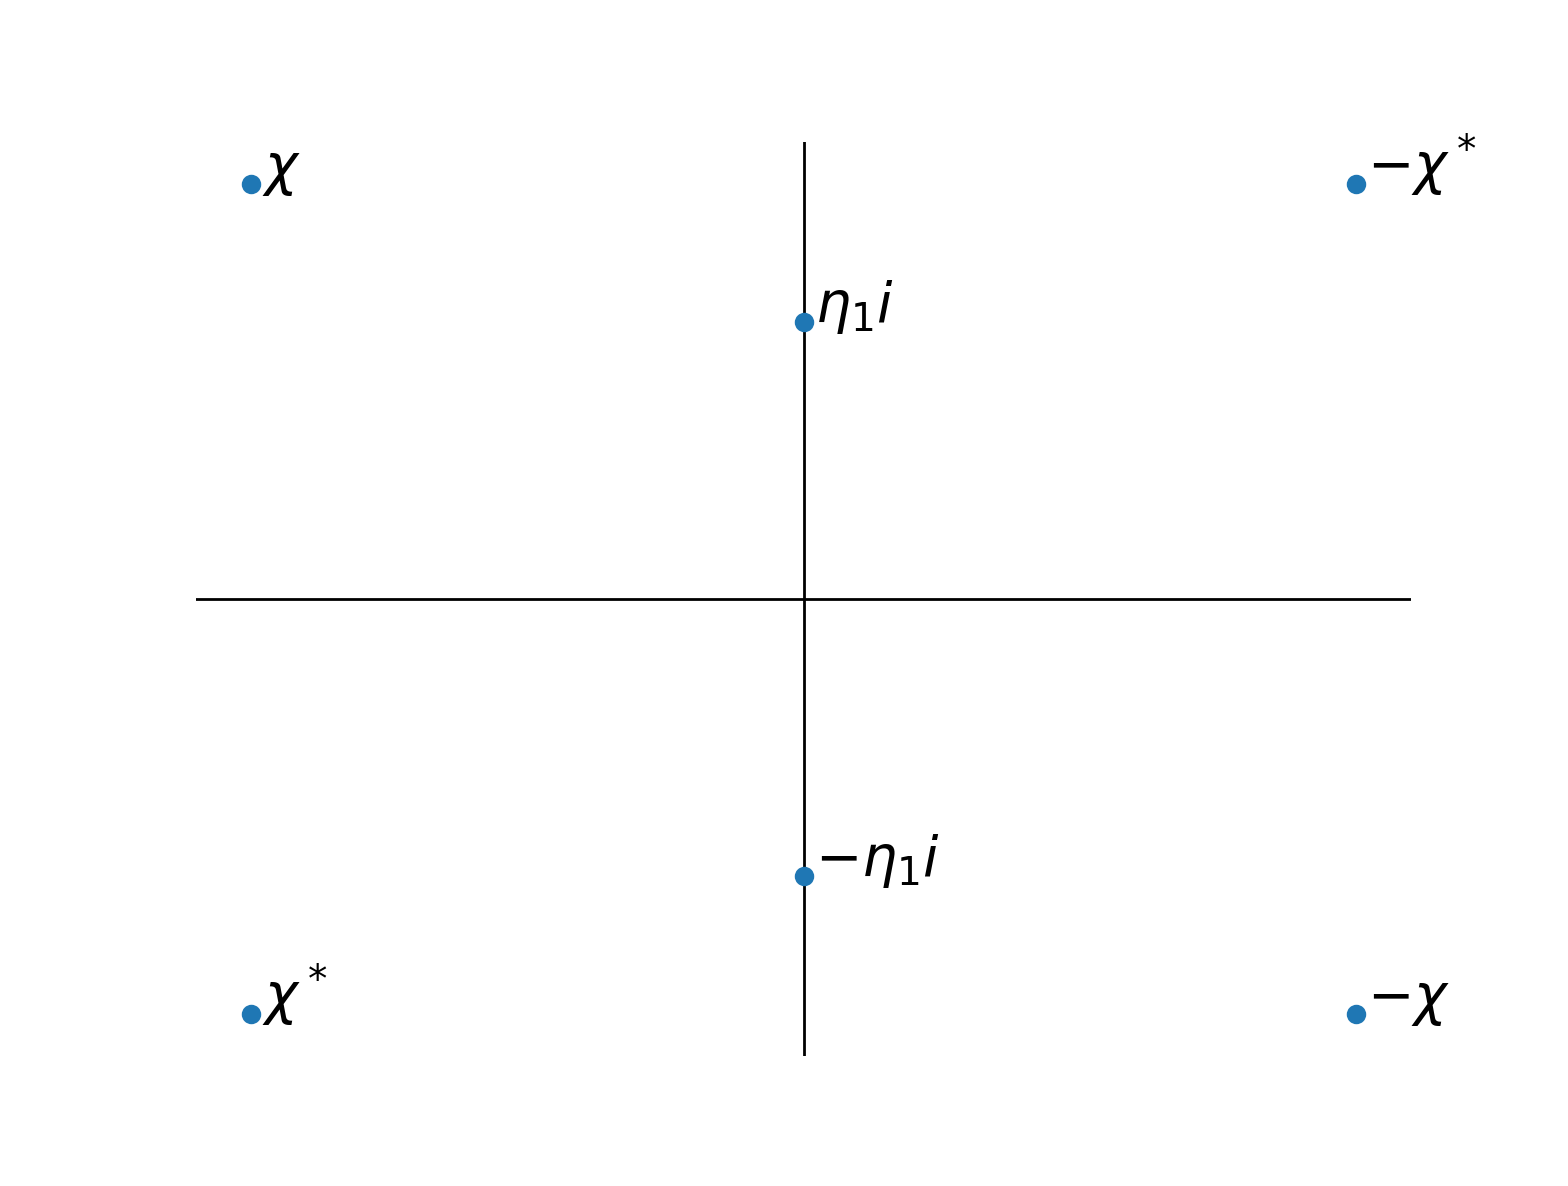
\includegraphics[width=0.5\textwidth]{pole_structure}
	\caption{\label{fig:pole_structure} The pole structure of the auto-correlation of the GLE Green's function $F(t)$ with an exponential memory kernel.}
\end{figure}

$\int\frac{dw}{2\pi} g\left(\omega\right) \left|\tilde{F}\left(\omega\right)\right|^2$ may now be evaluated using the residue theorem (closing the contour at $i\omega\rightarrow\infty$) provided that $g$ does not grow too fast as $\Im(\omega)\rightarrow\infty$. Assuming $g(\omega)$ has no poles and that $g(-\omega^*)=g(\omega)^*$ (which is useful for the purposes of this report),
\begin{equation}
	\int\frac{dw}{2\pi} g\left(\omega\right) \left|\tilde{F}\left(\omega\right)\right|^2 =  -\frac{1}{2 \tau^{2}}\left(\frac{1}{2 \chi' \chi''} \operatorname{Re}\left(\frac{g(\chi)}{\chi\left(\chi^{2}+\eta_{1}^{2}\right)}\right)+\frac{g(i\eta_{1})}{\left(|\chi|^{2}+n_{1}^{2}\right)^{2} \eta_{1}}\right) \label{eqn:integral_over_CF}
\end{equation}

\subsection{Evaluating the ISF and Energy Auto-correlation Function for an Exponential Memory Kernel}

Using equation \ref{eqn:integral_over_CF} the results derived in Section \ref{isf_gle_well} and \ref{kinetic_autocorrelation} can be evaluated for an exponential memory kernel $K(t)=\frac{1}{\tau}e^{-\frac{t}{\tau}}$. Substituting the expressions for the ISF and kinetic energy auto-correlation into equation \ref{eqn:integral_over_CF} and simplifying results in,
\begin{equation}
	ISF\left(\Delta \vec{K}, t\right) = ISF\left(\Delta \vec{K}, \infty\right) \exp\left(\frac{-\sigma^2\left|\Delta \vec{K}\right|^2}{2m^2\tau^2}\left(\frac{e^{-\chi''t}}{2\chi'\chi''}\operatorname{Re}\left(\frac{e^{i\chi't}}{\chi\left(\chi^2+\eta_1^2\right)}\right) + \frac{e^{-\eta_1t}}{\left(\left|\chi\right|^2+\eta_1^2\right)^2\eta_1}\right)\right) \label{isf_exp}
\end{equation}
\begin{equation}
	\left<E(0)E(t)\right>=\left<E(0)E(\infty)\right> + \frac{\sigma^4}{4\tau^4m^2}\left(\frac{e^{-\chi''t}}{2\chi'\chi''}\operatorname{Re}\left(\frac{\chi e^{i\chi't}}{\chi^2+\eta_1^2}\right) + \frac{\eta_1e^{-\eta_1 t}}{\left(\left|\chi\right|^2 + \eta_1^2\right)^2} \right)^2
\end{equation}
$$
\left<E(0)E(\infty)\right> = \frac{\sigma^4}{4\tau^4m^2}\left(\frac{1}{2\chi'\chi''}\operatorname{Re}\left(\frac{\chi}{\chi^2+\eta_1^2}\right) - \frac{\eta_1}{\left(\left|\chi\right|^2 + \eta_1^2\right)^2} \right)^2
$$

Where $\chi=:\chi'+\chi''i$.
